\documentclass[11pt,a4paper,twocolumn]{article}

% === Core Packages ===
\usepackage[margin=2cm]{geometry}
\usepackage[utf8]{inputenc}
\usepackage[T1]{fontenc}
\usepackage{times}
\usepackage{amsmath,amssymb}
\usepackage{graphicx}
\usepackage{booktabs}
\usepackage{float}
\usepackage{enumitem}
\usepackage{tikz}
\usepackage{pgfplots}
\pgfplotsset{compat=1.18}
\usetikzlibrary{arrows.meta,shapes.geometric,positioning,calc,decorations.markings,fit,backgrounds}

% === Citation (IEEE style) ===
\usepackage[numbers,sort&compress]{natbib}
\bibliographystyle{IEEEtranN}

% === Hyperref ===
\usepackage[hidelinks]{hyperref}
\usepackage{xurl}

% === Settings ===
\setlength{\parindent}{1em}
\setlength{\parskip}{0.3em}

% === Title ===
\title{\textbf{Zdecentralizowana sieć reputacji:\\Ramy naturalnej organizacji społecznej}}
\author{Pavel Kudrna\\Prague, Czechia\\Draft v1 --- March 2026}
\date{}

\begin{document}
\maketitle

% ============================================================
% ABSTRACT
% ============================================================
\begin{abstract}
Poczucie sprawiedliwości---przekonanie, że krzywdy zostają naprawione, a zasługi nagrodzone---jest najsilniejszą siłą spajającą społeczeństwo. Gdy scentralizowane instytucje władzy nie potrafią zapewnić tego poczucia, ponieważ koszt wyegzekwowania prawa przewyższa wartość samego prawa, spójność społeczna ulega erozji. Obecne struktury instytucjonalne nie potrafią rozstrzygnąć znaczącej klasy sporów w sposób systematycznie taki sam, w jaki centralne planowanie zawodzi przy alokacji zasobów: poprzez asymetrię informacji, brak pętli sprzężenia zwrotnego oraz oderwanie decydentów od konsekwencji ich decyzji. Niniejsza praca przedstawia Reputacyjną Sieć Społeczną (RSN): zdecentralizowaną, niepodatną na korupcję i odporną na cenzurę warstwę komunikacyjną zbudowaną na Zdecentralizowanych Identyfikatorach (DID), która umożliwia pseudonimowym uczestnikom publikowanie, weryfikowanie i konsumowanie informacji reputacyjnych o zachowaniach w świecie rzeczywistym. Podstawowy mechanizm opiera się na trzech zasadach projektowych: (1)~asymetrycznej strukturze kosztów, w której odczyt danych reputacyjnych jest tani, ale zapis wymaga weryfikowalnego wysiłku; (2)~niedeterministycznym protokole wyboru weryfikatora opartym na spójnym haszowaniu, który wycenia radykalne twierdzenia poprzez rosnące koszty iteracji; oraz (3)~rynkowym modelu autorytetu reputacyjnego, w którym prywatni weryfikatorzy stawiają zgromadzoną reputację na dokładność twierdzeń, które popierają. Powstała architektura wytwarza emergentną merytokrację bez centralnej koordynacji i umożliwia stopniową, odwracalną ścieżkę migracji z istniejących systemów administrowanych przez państwo.
\end{abstract}

% ============================================================
% 1. INTRODUCTION
% ============================================================
\section{Wprowadzenie}

\subsection{Problem scentralizowanego zaufania}

Współczesne rządzenie opiera się na fundamentalnym założeniu: że scentralizowane instytucje potrafią pośredniczyć w zaufaniu między obcymi na dużą skalę. Sądy rozstrzygają spory. Rejestry poświadczają własność. Organy regulacyjne egzekwują standardy. Instytucje te zaprojektowano w epoce, gdy informacja była rzadka, komunikacja powolna, a delegowanie władzy do centralnego organu było jedynym wykonalnym mechanizmem koordynacji. Scentralizowane rządzenie zawodzi jednak z tych samych strukturalnych powodów co centralne planowanie: asymetrii informacji, braku pętli sprzężenia zwrotnego oraz oderwania decydentów od konsekwencji ich decyzji.

Założenie to zawodzi na przykład wtedy, gdy koszt instytucjonalnego pośrednictwa przewyższa wartość sporu. Rozważmy najemcę, który odkrywa, że jego wynajmowane mieszkanie nie posiada prawnie wymaganego certyfikatu bezpieczeństwa instalacji elektrycznej---stanu stwarzającego bezpośrednie zagrożenie życia. Prawo najemcy do odstąpienia od umowy jest jednoznaczne. Jednak koszt wyegzekwowania tego prawa na drodze sądowej przewyższa wartość pieniężną kaucji i należnych odszkodowań, nawet wliczając potencjalne ustawowe zadośćuczynienie~\cite{czcourtfees}. Racjonalną reakcją jest pogodzenie się ze stratą i wycofanie się.

Nie jest to patologiczny przypadek skrajny. To domyślne doświadczenie znaczącej klasy sporów, w których szkoda jest realna, ale stawki pieniężne spadają poniżej progu, przy którym instytucjonalne egzekwowanie staje się ekonomicznie racjonalne. Efektem jest system strukturalnie sprzyjający złym aktorom: ci, którzy krzywdzą innych w wolumenach poniżej tego progu, mogą działać bezkarnie, ponieważ koszt dochodzenia sprawiedliwości spada na stronę poszkodowaną.

Powyższy przykład zaczerpnięto ze środowiska prawnego autora---czeskiego systemu prawa cywilnego. W innych tradycjach prawnych---prawie precedensowym common law, prawie zwyczajowym, systemach mieszanych---sprawiedliwość zawodzi w różny sposób i w różnym stopniu, w zależności od kulturowej i proceduralnej specyfiki danej jurysdykcji. Czytelnicy zapewne rozpoznają równoważne przykłady z własnego kontekstu. Strukturalnie uniwersalny jest wzorzec: spory, których wartość spada poniżej progu ekonomicznie racjonalnego egzekwowania, kończą się przejęciem straty przez stronę poszkodowaną. RSN nie obiecuje doskonałej sprawiedliwości---jedynie zmniejsza strukturalną przewagę, jaką cieszą się źli aktorzy, gdy instytucjonalne egzekwowanie jest nieopłacalne.

\subsection{Dlaczego istniejące rozwiązania są niewystarczające}

\textbf{Ramy Zdecentralizowanej Tożsamości (DID)}~\cite{did2022} zapewniają mechanizmy kryptograficzne do samodzielnego zarządzania tożsamością, lecz koncentrują się głównie na weryfikacji tożsamości, nie odnosząc się do szerszej kwestii reputacji behawioralnej.

\textbf{Soulbound Tokens (SBT)}~\cite{weyl2022} ujmują spostrzeżenie, że reputacja jest nieprzenoszalna, ale opierają się na infrastrukturze blockchain z ograniczeniami skalowalności i nie odnoszą się do bodźców ekonomicznych regulujących wprowadzanie informacji. Pokrewne koncepcje, takie jak tokeny zasług (np. Liberland), podzielają podobną filozofię, lecz pozostają związane z konkretnymi ramami jurysdykcyjnymi.

\textbf{Zdecentralizowane Organizacje Autonomiczne (DAO)}~\cite{buterin2014} realizują zarządzanie poprzez inteligentne kontrakty, ale odtwarzają plutokratyczną dynamikę, w której wpływ jest proporcjonalny do kapitału. Głosowanie kwadratowe~\cite{buterin2019} częściowo to łagodzi, lecz ogranicza praktyczną adopcję. DAO stają również w obliczu fundamentalnego \emph{problemu wyroczni}: inteligentne kontrakty nie potrafią wiarygodnie weryfikować stanów świata rzeczywistego bez zaufanego zewnętrznego źródła, a problem ten nie ma ogólnego rozwiązania w ramach architektury blockchain.

Żaden istniejący system nie łączy decentralizacji, odporności na cenzurę, pseudonimowości, weryfikowalnego kosztu wejścia i emergentnego konsensusu.

\subsection{Wkład}

Niniejsza praca wnosi następujący wkład:
\begin{enumerate}[nosep]
\item Definicję \textbf{Reputacyjnej Sieci Społecznej (RSN)}, zdecentralizowanego protokołu rozszerzającego ramy DID o wsparcie dwustronnej wymiany reputacji.
\item \textbf{Niedeterministyczny protokół wyboru weryfikatora} oparty na spójnym haszowaniu~\cite{karger1997}.
\item \textbf{Zasadę Kosztownego Radykalizmu}, wyceniającą twierdzenia według ich odległości od konsensusu sieci przez trzy nakładające się kanały kosztowe.
\item \textbf{Model Reputowanego Autorytetu} z asymetrycznymi bodźcami, gdzie fałszywe poparcie kosztuje katastrofalnie więcej niż uczciwe opłaty.
\item \textbf{Stopniową ścieżkę migracji} poprzez równoległą infrastrukturę fiskalną.
\end{enumerate}

% ============================================================
% 2. DESIGN PRINCIPLES
% ============================================================
\section{Zasady projektowe}

Architektura RSN jest ograniczona pięcioma nienegocjowalnymi zasadami projektowymi.

\textbf{Ciągłość i ewolucja.} System współistnieje z istniejącymi instytucjami przez okres przejściowy o nieokreślonej długości. Przejście musi być odwracalne na każdym etapie.

\textbf{Dobrowolność i odpowiedzialność.} Uczestnictwo jest dobrowolne, ale dobrowolność jest sprzężona z odpowiedzialnością: uczestnik przejmujący kontrolę nad funkcją instytucjonalną jednocześnie przejmuje związane z nią obowiązki.

\textbf{Różnorodność i neutralność kulturowa.} Konsensus wyłania się z dwustronnych interakcji, a nie z gotowych reguł narzuconych przez projektantów systemu.

\textbf{Odporność i odporność na cenzurę.} Koszt cenzurowania sieci musi przewyższać koszt jej tolerowania. Tylko pełny totalitaryzm---za rujnującą cenę polityczną i ekonomiczną---może stłumić system.

\textbf{Konsensus i egzekwowanie.} System uwzględnia ludzkie skłonności do małostkowości, złośliwości i satysfakcji z odwetu jako cechy nośne. Występek nie jest zakazany; jest wyceniany.

% ============================================================
% 3. SYSTEM OVERVIEW
% ============================================================
\section{Przegląd systemu}

\subsection{Reputacyjna Sieć Społeczna}

RSN to zdecentralizowana warstwa komunikacyjna typu peer-to-peer, w której uczestnicy wymieniają weryfikowalne informacje o zachowaniach w świecie rzeczywistym. Jej definiujące właściwości to: zdecentralizowana i niecenzurowalna infrastruktura; pseudonimowe uczestnictwo poprzez DID; asymetryczna struktura kosztów (odczyt jest tani, zapis kosztowny); weryfikowalność kryptograficzna; oraz \textbf{wsparcie standardów}---formaty czytelne maszynowo dla informacji propagowanych przez sieć, dla usług oferowanych przez autorytety (kompozycja twierdzeń, poparcie, usługa świadka) oraz dla formatu polityki obejmującego reguły oceny reputacji kontrahenta i szacowania ryzyka niezgodności polityki (między deklarowanym a rzeczywistym zachowaniem).

\subsection{Komponenty architektoniczne}

RSN składa się z czterech głównych komponentów (Rys.~\ref{fig:architecture}):
\begin{enumerate}[nosep]
\item \textbf{Warstwa DID.} Tożsamości uczestników z deklarowanymi regułami, metadanymi reputacji i routingiem sieciowym.
\item \textbf{Protokół Twierdzeń.} Ustrukturyzowany format publikowania stwierdzeń o zdarzeniach w świecie rzeczywistym.
\item \textbf{Sieć Weryfikacyjna.} Zdecentralizowany protokół przydzielania weryfikatorów przy użyciu spójnego haszowania.
\item \textbf{Warstwa Agregacji Reputacji.} Usługi wytwarzające czytelne dla człowieka podsumowania reputacji.
\end{enumerate}

\begin{figure}[ht]
\centering
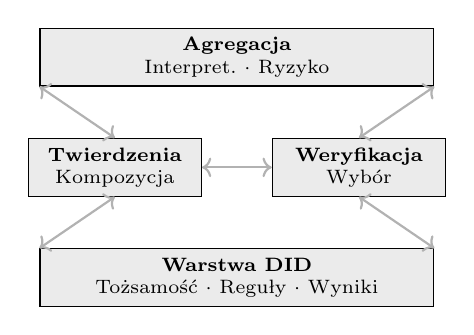
\begin{tikzpicture}[
    layer/.style={draw, minimum height=0.7cm, align=center, font=\scriptsize, fill=black!8},
    arr/.style={<->, thick, gray!60}
]
\node[layer, minimum width=5cm] (agg) at (0,2.8) {\textbf{Agregacja}\\Interpret.\ $\cdot$ Ryzyko};
\node[layer, minimum width=2.2cm] (claim) at (-1.55,1.4) {\textbf{Twierdzenia}\\Kompozycja};
\node[layer, minimum width=2.2cm] (verif) at (1.55,1.4) {\textbf{Weryfikacja}\\Wybór};
\node[layer, minimum width=5cm] (did) at (0,0) {\textbf{Warstwa DID}\\Tożsamość $\cdot$ Reguły $\cdot$ Wyniki};

\draw[arr] (agg.south west) -- (claim.north);
\draw[arr] (agg.south east) -- (verif.north);
\draw[arr] (claim.east) -- (verif.west);
\draw[arr] (claim.south) -- (did.north west);
\draw[arr] (verif.south) -- (did.north east);
\end{tikzpicture}
\caption{Czterowarstwowa architektura RSN.}
\label{fig:architecture}
\end{figure}

\subsection{Role uczestników}

Transakcja weryfikacyjna angażuje do sześciu odrębnych ról DID (Rys.~\ref{fig:roles}): \textbf{Wystawca} ($DID_I$, tworzy i przesyła twierdzenie), \textbf{Podmiot} ($DID_S$, DID, którego dotyczy twierdzenie---może pokrywać się z Wystawcą), \textbf{Autorytet} ($DID_A$, popiera twierdzenie za opłatą; może również oferować usługi świadka---\emph{opcjonalnie}), \textbf{Świadek} ($DID_{W_{1..n}}$, incognito monitorujący uczciwość weryfikatora za pomocą kodów wyzwań---\emph{opcjonalnie}), \textbf{Weryfikator} ($DID_V$, algorytmicznie wybrany do publikacji twierdzenia) oraz \textbf{RSN} (sieć, w której publikowane są zweryfikowane twierdzenia). Każda rola może zostać delegowana innemu DID (Rozdział~7.4). Autorytet zwykle łączy poparcie z usługami świadka, ale obie funkcje są logicznie niezależne.

\begin{figure}[ht]
\centering
\begin{tikzpicture}[
    role/.style={draw, rounded corners, minimum width=1.1cm, minimum height=0.45cm, align=center, font=\scriptsize, fill=black!8},
    opt/.style={draw, rounded corners, minimum width=1.1cm, minimum height=0.45cm, align=center, font=\scriptsize, fill=black!8, dashed},
    arr/.style={-{Stealth[length=3pt]}, thick},
    oarr/.style={-{Stealth[length=3pt]}, thick, dashed, gray},
    lbl/.style={font=\tiny, fill=white, inner sep=1pt}
]
\node[role] (I) at (0,2.4) {\textbf{Wystawca}};
\node[role] (S) at (-2.5,2.4) {\textbf{Podmiot}};
\node[opt] (A) at (2.5,1.2) {\textbf{Autorytet}};
\node[opt] (W) at (-2.5,0) {\textbf{Świadek}};
\node[role] (V) at (2.5,-0.6) {\textbf{Weryfikator}};
\node[role, fill=black!5, draw=gray] (N) at (0,-1.8) {RSN};

\draw[arr] (I) -- node[lbl] {o} (S);
\draw[oarr] (I) -- node[lbl,sloped] {popiera} (A);
\draw[oarr] (I) -- node[lbl,sloped] {wyzwanie} (W);
\draw[arr] (I) -- node[lbl,sloped] {żądanie} (V);
\draw[oarr] (W) -- node[lbl] {monitoruje} (V);
\draw[arr] (V) -- node[lbl] {publikuje} (N);
\end{tikzpicture}
\caption{Role DID w transakcji weryfikacyjnej. Przerywana = opcjonalna (Autorytet, Świadek).}
\label{fig:roles}
\end{figure}

\subsection{Niepodatność na korupcję: cztery siły}

Niepodatność RSN na korupcję nie wynika z pojedynczego mechanizmu, lecz z czterech równoczesnych sił. Żadna nie wystarcza samodzielnie; dopiero ich połączenie czyni próbę korupcji ekonomicznie irracjonalną.

\textbf{Nieprzewidywalny cel.} Weryfikator dla każdego twierdzenia jest wybierany niedeterministycznie poprzez spójne haszowanie (Rozdział~5.3). Atakujący nie może z góry namierzyć konkretnego weryfikatora do przekupienia, ponieważ tożsamość weryfikatora jest funkcją treści twierdzenia i poprzednich iteracji, a nie wyboru wystawcy.

\textbf{Dźwignia reputacyjna---w górę powoli, w dół szybko.} Reputację można zdobywać jedynie stopniowo, poprzez trwałe konsekwentne zachowanie. Można ją jednak katastrofalnie utracić w jednym oszukańczym poparciu (Rozdział~6.2). Ta asymetria oznacza, że lata zgromadzonej reputacji mogą zostać zniszczone przez jedno nieuczciwe poparcie; optymalną strategią pozostaje odrzucanie podejrzanych twierdzeń.

\textbf{Publiczna obietnica.} Każdy Posiadacz DID publicznie deklaruje swoją politykę---czytelny maszynowo zestaw reguł, których zobowiązuje się przestrzegać. Rozbieżność między deklaracją a rzeczywistym zachowaniem jest wykrywalna i wyceniana jako przewinienie reputacyjne poważniejsze niż samo naruszenie (Rozdział~7.3). Hipokryzja jest zatem kosztowniejsza niż bezpośrednia nieuczciwość.

\textbf{Asymetria kosztu ataku na siatkę.} Koszt cenzurowania lub destabilizowania sieci rośnie nieliniowo wraz z rozmiarem i gęstością sieci, podczas gdy koszt jej tolerowania pozostaje stały. Aby cenzura się opłaciła, scentralizowany aktor musiałby zastosować ją w całej sieci---co wymaga środków nieproporcjonalnych do jakiejkolwiek wyobrażalnej korzyści (Rozdział~10).

% ============================================================
% 4. DECENTRALIZED IDENTITY MODEL
% ============================================================
\section{Model zdecentralizowanej tożsamości}

\subsection{DID o szczególnych właściwościach}

RSN rozszerza specyfikację W3C DID Core~\cite{did2022} o: \textbf{Deklarowane Reguły} (czytelne maszynowo zobowiązania behawioralne), \textbf{Metadane Reputacji} (zagregowany wynik behawioralny) oraz \textbf{Routing Sieciowy} (zmienna brama onion odrębna od stabilnej pozycji na pierścieniu).

\subsection{Cykl życia twierdzenia}

Twierdzenie przechodzi przez sześć etapów (Rys.~\ref{fig:lifecycle}): kompozycja, opcjonalne poparcie autorytetu, wybór weryfikatora poprzez spójne haszowanie, decyzja weryfikacyjna (akceptacja lub odrzucenie z iteracją), publikacja oraz aktualizacja reputacji wszystkich stron.

\begin{figure}[ht]
\centering
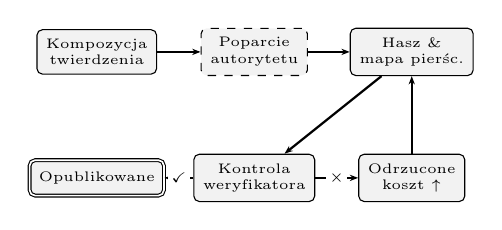
\begin{tikzpicture}[
    stp/.style={draw, rounded corners=2pt, minimum width=1.3cm, minimum height=0.45cm, align=center, font=\tiny, fill=black!5},
    arr/.style={-{Stealth[length=3pt]}, thick},
    lbl/.style={font=\tiny, fill=white, inner sep=1pt}
]
\node[stp] (comp) at (0,0) {Kompozycja\\twierdzenia};
\node[stp, dashed] (auth) at (2.0,0) {Poparcie\\autorytetu};
\node[stp] (hash) at (4.0,0) {Hasz \&\\mapa pierśc.};
\node[stp] (ver) at (2.0,-1.6) {Kontrola\\weryfikatora};
\node[stp, double] (pub) at (0,-1.6) {Opublikowane};
\node[stp] (rej) at (4.0,-1.6) {Odrzucone\\koszt $\uparrow$};

\draw[arr] (comp) -- (auth);
\draw[arr] (auth) -- (hash);
\draw[arr] (hash) -- (ver);
\draw[arr] (ver) -- node[lbl] {\checkmark} (pub);
\draw[arr] (ver) -- node[lbl] {$\times$} (rej);
\draw[arr] (rej) -- ++(0,0.8) -| (hash);
\end{tikzpicture}
\caption{Cykl życia twierdzenia z pętlą iteracji.}
\label{fig:lifecycle}
\end{figure}

\subsection{Relacja do W3C DID Core}

Model tożsamości RSN jest właściwym nadzbiorem specyfikacji W3C DID Core~\cite{did2022}. Wszystkie DID w RSN są prawidłowymi DID W3C. Rozszerzenia specyficzne dla RSN są zakodowane jako właściwości dokumentu DID zdefiniowane w dedykowanej specyfikacji metody DID, kompatybilnej z istniejącą infrastrukturą, taką jak ION~\cite{buchner2021} i Ceramic~\cite{ceramic2023}.

% ============================================================
% 5. VERIFICATION AND PROPAGATION
% ============================================================
\section{Weryfikacja i propagacja informacji}

\subsection{Koszt wprowadzenia informacji}

Podstawową zasadą ekonomiczną RSN jest asymetria między odczytem a zapisem. Odczyt danych reputacyjnych zbliża się do zerowego kosztu krańcowego dla uczestników należących do sieci DID i posiadających dostęp współmierny do ich reputacji---nowicjusze muszą stopniowo wypracowywać szerszy dostęp (zob. zapobieganie pasożytnictwu). Zapis---rozumiany jako trwałe zmaterializowanie reputacji w sieci, a nie jako jednorazowy akt techniczny---wymaga weryfikowalnej skumulowanej inwestycji w trzech wymiarach: \textbf{czasu} (lat życia poświęconych konsekwentnemu zachowaniu, dotrzymanym zobowiązaniom i pielęgnowanym relacjom), \textbf{energii} (wysiłku włożonego w uczciwe postępowanie, dbałość o partnerstwa i długoterminową wiarygodność) oraz \textbf{pieniędzy} (inwestycji we własne imię---rozwoju zawodowego, jakości własnej pracy, restytucji za wyrządzone krzywdy). Reputacji nie da się kupić natychmiast---jest ona wynikiem gromadzenia trwającego całe życie, które system jedynie uwidacznia i czyni przenaszalnym między kontekstami. Jednorazowe koszty techniczne protokołu (podpisy kryptograficzne, opłaty weryfikatorów) są znikome w porównaniu z tą podstawową inwestycją.

\subsection{Graf społeczny i głębokość kontaktów}

RSN jest fundamentalnie siecią społeczną: każdy DID dodaje kontakty (inne DID), które zezwalają na połączenie. Kontakty te mają własne kontakty i tak dalej. Algorytmiczne wyszukiwanie weryfikatora działa w konfigurowalnej głębokości $h$ powiązanych kontaktów (np. $h=3$: własne bezpośrednie kontakty, ich kontakty oraz kontakty kontaktów). Ta architektura nie wymaga jednego globalnego blockchaina---naturalnie sprzyja wyłanianiu się społeczności/klastrów z nakładaniami na inne społeczności. Każdy uczestnik DID musi mieć opublikowaną \textbf{politykę}---czytelny maszynowo zestaw reguł regulujących sposób oceny przychodzących żądań. Naruszenia polityki są zapisywane w sieci jako negatywne artefakty.

\subsection{Algorytmiczny wybór weryfikatora}

Protokół weryfikacji wykorzystuje spójne haszowanie~\cite{karger1997} (Rys.~\ref{fig:verifier}). Weryfikacja jest usługą płatną: weryfikatorzy działają za opłatą, tworząc rynek, w którym konkurencja napędza cenę, szybkość i niezawodność.

\textbf{Krok 1.} Dokument twierdzenia jest łączony z wynikiem haszu poprzedniej iteracji (lub $\varnothing$ przy pierwszej iteracji) i haszowany:
\begin{equation}
\text{pos} = f_h(\text{claim} \| \text{prev\_hash})
\label{eq:hash}
\end{equation}

Algorytm musi obejmować \emph{pełną ścieżkę} wszystkich poprzednich żądań i odpowiedzi---nie tylko hasz poprzedniej iteracji. Pełna odpowiedź każdego weryfikatora (akceptacja, odrzucenie, podana cena, powód) jest dołączana do rosnącego dokumentu, weryfikowalna poprzez podpisy kryptograficzne na każdym kroku.

\textbf{Krok 2.} Hasz jest mapowany na $N$ pozycji na pierścieniu spójnego haszu, równomiernie rozłożonych (np. dla $N=4$: $+0^{\circ}, +90^{\circ}, +180^{\circ}, +270^{\circ}$). Z każdej pozycji wyszukiwanie zgodne z ruchem wskazówek zegara wybiera najbliższy DID jako kandydata na weryfikatora (Rys.~\ref{fig:multipoint}). $N$ jest parametrem zmiennym, który może zależeć od odsetka aktualnie aktywnych DID, pory dnia lub historycznej responsywności sieci.

\textbf{Krok 3.} Weryfikator akceptuje (publikuje, stawiając reputację) lub odrzuca (wracając do Kroku~1 z haszem odrzucenia). Gdy węzeł nie odpowiada mimo deklarowania statusu online, kolejne żądanie musi zawierać wszystkie odpowiedzi wszystkich $N$ poprzednich kandydatów na weryfikatorów.

\textbf{Zapobieganie pasożytnictwu.} Docelowe DID mogą ustalać opłaty lub ograniczenia dostępu dla zapytań od nowych DID o niewielkiej reputacji. Ten stopniowalny mechanizm (nie binarny) zmusza nowicjuszy do budowania reputacji poprzez rzeczywistą aktywność, zanim zaczną swobodnie konsumować dane innych.

\begin{figure}[ht]
\centering
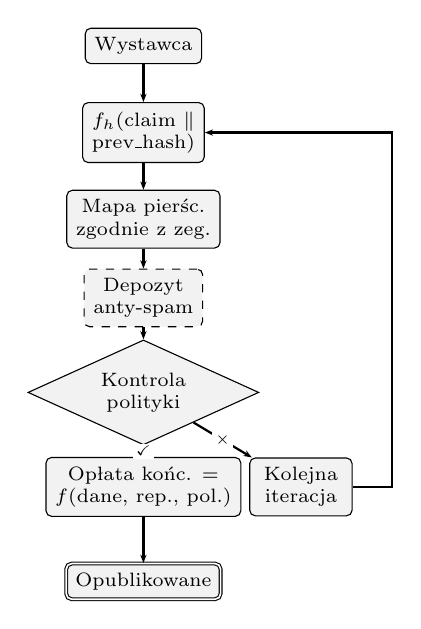
\begin{tikzpicture}[
    box/.style={draw, rounded corners=2pt, minimum width=1.3cm, minimum height=0.45cm, align=center, font=\scriptsize, fill=black!5},
    dec/.style={draw, diamond, aspect=2.2, minimum width=0.9cm, align=center, font=\scriptsize, fill=black!5},
    arr/.style={-{Stealth[length=3pt]}, thick},
    lbl/.style={font=\tiny, fill=white, inner sep=1pt}
]
\node[box] (iss) at (0,0) {Wystawca};
\node[box] (hash) at (0,-1.1) {$f_h$(claim $\|$\\prev\_hash)};
\node[box] (ring) at (0,-2.2) {Mapa pierśc.\\zgodnie z zeg.};
\node[box, dashed] (spam) at (0,-3.2) {Depozyt\\anty-spam};
\node[dec] (check) at (0,-4.4) {Kontrola\\polityki};
\node[box] (rej) at (2,-5.6) {Kolejna\\iteracja};
\node[box] (fee) at (0,-5.6) {Opłata końc. =\\$f$(dane, rep., pol.)};
\node[box, double] (pub) at (0,-6.8) {Opublikowane};

\draw[arr] (iss) -- (hash);
\draw[arr] (hash) -- (ring);
\draw[arr] (ring) -- (spam);
\draw[arr] (spam) -- (check);
\draw[arr] (check) -- node[lbl] {$\times$} (rej);
\draw[arr] (check) -- node[lbl] {\checkmark} (fee);
\draw[arr] (fee) -- (pub);
\draw[arr] (rej.east) -- ++(0.5,0) |- (hash.east);
\end{tikzpicture}
\caption{Protokół wyboru weryfikatora. Depozyt anty-spam jest opcjonalny i może być zwrotny. Opłata końcowa jest płatna tylko przy akceptacji.}
\label{fig:verifier}
\end{figure}

Każde odrzucenie dołącza pełną odpowiedź weryfikatora (wraz z powodami i warunkami) do dokumentu twierdzenia, rozszerzając jego treść. Z rozszerzonego dokumentu niedeterministycznie obliczany jest nowy hasz, mapowany na inną pozycję na pierścieniu i wybierający innego weryfikatora. Dokumentacja pełnej ścieżki jest obowiązkowa---wystawca nie może przewidzieć ani wpłynąć na kolejnego weryfikatora. Jeśli weryfikator zignoruje żądanie mimo zgodnej deklarowanej polityki, świadkowie (jeśli obecni) to rejestrują, a wystawca może dołączyć dowody świadków przy końcowej publikacji.

\begin{figure}[ht]
\centering
\begin{tikzpicture}[scale=0.65]
% Ring
\draw[thick] (0,0) circle (2.2cm);
% DID nodes on ring
\foreach \a in {10,55,80,120,150,195,230,260,305,340} {
  \fill[black!40] (\a:2.2) circle (1.5pt);
}
% Hash offset arrow pointing to initial position
\draw[-{Stealth[length=3pt]}, thick, black!60] (0,0) -- node[font=\tiny,above,sloped,pos=0.6] {$f_h$} (37:2.2);
\fill[black] (37:2.2) circle (2pt);
\node[font=\tiny,anchor=south west] at (37:2.35) {$h_0$};
% N=4 points offset from h0 by +0, +90, +180, +270
\foreach \offset/\l in {0/P1,90/P2,180/P3,270/P4} {
  \pgfmathsetmacro{\ang}{37+\offset}
  \node[fill=black, circle, inner sep=1.5pt] (p\offset) at (\ang:2.2) {};
  \node[font=\tiny,font=\bfseries] at (\ang:2.75) {\l};
  % clockwise search arc
  \draw[-{Stealth[length=2.5pt]}, thick, gray] (\ang:2.2) arc (\ang:\ang+30:2.2);
}
\node[font=\scriptsize, align=center] at (0,0) {Pierścień\\haszu};
\node[font=\tiny, align=center] at (0,-3.2) {$h_0 = f_h(\text{claim})$, następnie $+0^{\circ},+90^{\circ},+180^{\circ},+270^{\circ}$\\Każdy punkt $\rightarrow$ wyszukiwanie zgodne z zegarem};
\end{tikzpicture}
\caption{Wybór wielopunktowy ($N{=}4$). Hasz $h_0$ ustala przesunięcie; 4 punkty równomiernie rozłożone od $h_0$.}
\label{fig:multipoint}
\end{figure}

\subsection{Protokół świadka}

Rola \textbf{Świadka} zapewnia incognito rozliczalność uczciwości weryfikatora poprzez kryptograficzny protokół kodów wyzwań:

\textbf{Krok W1.} Żądający podpisuje żądanie weryfikacji i wysyła je do $N_w$ świadków---kontaktów z sieci społecznej żądającego lub wyspecjalizowanych dostawców usług świadka działających za opłatą.

\textbf{Krok W2.} Każdy świadek $w_i$ podpisuje całe podpisane żądanie, zachowuje oryginalny podpis $\sigma_i$ i oblicza kod wyzwania $c_i = h(\sigma_i)$. Kod wyzwania jest dołączany do żądania.

\textbf{Krok W3.} Żądanie, niosące teraz $N_w$ kodów wyzwań, jest wysyłane do weryfikatora. Weryfikator obserwuje kody, ale \emph{nie może ustalić}, kim są świadkowie ani czy kody odpowiadają prawdziwym podpisom.

\textbf{Krok W4 (uczciwy weryfikator).} Jeśli weryfikator odpowiada zgodnie ze swoją deklarowaną polityką, kody wyzwań pozostają nieprzejrzyste. Świadkowie nigdy nie zostają ujawnieni. Nie są publikowane żadne dodatkowe dane.

\textbf{Krok W5 (naruszenie polityki).} Jeśli weryfikator narusza swoją politykę (ignoruje żądanie, odpowiada niekonsekwentnie), żądający posiada oryginalne podpisy świadków $\sigma_i$. Można je opublikować jako dane towarzyszące: każdy może zweryfikować $c_i = h(\sigma_i)$, dowodząc, że świadek był obecny. Żądający może opublikować niezależnie---weryfikator już podpisał kody wyzwań w swojej odpowiedzi.

\textbf{Właściwość blefu.} Żądający może podstawić losowe wartości za niektóre lub wszystkie kody wyzwań. Weryfikator nie potrafi odróżnić prawdziwych kodów (zabezpieczonych przez autorytety o wysokiej reputacji) od szumu. Ta \emph{niepewność} jest mechanizmem egzekwowania: każde żądanie niesie ryzyko, że szanowany autorytet obserwuje incognito. Koszt utrzymania tej presji jest bliski zeru (generowanie liczb losowych), podczas gdy potencjalny koszt nieuczciwości dla weryfikatora jest katastrofalny. Uczciwe zachowanie jest motywowane nawet przy braku rzeczywistych świadków.

\textbf{Autorytet jako świadek.} Autorytet popierający twierdzenie może połączyć usługi świadka: ,,Popieram twoje twierdzenie i pełnię rolę incognito świadka podczas weryfikacji''. Jest to naturalny model biznesowy---autorytet już posiada kontekst. Obie role są jednak logicznie niezależne.

\subsection{Zasada Kosztownego Radykalizmu}

Trzy kanały kosztowe nakładają się jednocześnie (Rys.~\ref{fig:radicalism}):

\textbf{Kanał 1: Koszt iteracji.} Każde odrzucenie wymusza nową iterację pochłaniającą czas i zasoby. Wzrost liniowy.

\textbf{Kanał 2: Rozrost dokumentu.} Każda iteracja dodaje pełną odpowiedź weryfikatora do dokumentu twierdzenia. Wzrost jest liniowy, ale z przesunięciem bazowym: początkowy ładunek (treść twierdzenia, poparcie autorytetu, podpisy kryptograficzne) ma już nietrywialny rozmiar $B_0$. Całkowity rozmiar po $k$ iteracjach: $S(k) = B_0 + k \cdot \Delta$, gdzie $\Delta$ to średni rozmiar odpowiedzi.

\textbf{Kanał 3: Premia za ryzyko weryfikatora.} Ryzyko jest subiektywne. Weryfikator ocenia, czy deklarowane polityki żądającego DID kolidują z jego własnymi interesami handlowymi, społecznymi lub politycznymi. Premia może rosnąć wykładniczo wraz z postrzeganą odległością od ,,ideału'' weryfikatora: $P(d) = \alpha \cdot e^{\beta d}$, gdzie $d$ to subiektywna metryka odległości weryfikatora. Poza osobistą granicą no-go weryfikator może odmówić całkowicie.

\begin{figure}[ht]
\centering
\begin{tikzpicture}
\begin{axis}[
    width=\columnwidth,
    height=4.5cm,
    xlabel={\footnotesize Radykalizm},
    ylabel={\footnotesize Koszt względny (log)},
    ymode=log,
    xmin=0, xmax=100,
    ymin=1, ymax=10000,
    grid=major,
    grid style={gray!20},
    legend style={at={(0.03,0.97)},anchor=north west,font=\tiny,draw=gray!50},
    tick label style={font=\tiny},
    label style={font=\footnotesize},
]
\addplot[black, thick, domain=0:100, samples=50] {1 + 0.3*x};
\addlegendentry{Koszt iteracji (liniowy)}
\addplot[black, thick, dashed, domain=0:100, samples=50] {1 + 0.15*x};
\addlegendentry{Rozrost dokumentu (liniowy)}
\addplot[black, thick, dotted, line width=1.2pt, domain=0:100, samples=100] {exp(0.08*x)};
\addlegendentry{Premia za ryzyko (wykładnicza)}
\end{axis}
\end{tikzpicture}
\caption{Eskalacja kosztów w trzech kanałach. Premia za ryzyko dominuje przy wysokim radykalizmie.}
\label{fig:radicalism}
\end{figure}

Co kluczowe, nie jest to cenzura. Żadne twierdzenie nie jest zakazane. System wycenia ryzyko (Tabela~\ref{tab:costs}).

\begin{table}[ht]
\centering
\caption{Porównanie kosztów według typów twierdzeń.}
\label{tab:costs}
\footnotesize
\begin{tabular}{@{}lcccc@{}}
\toprule
\textbf{Typ} & \textbf{Iter.} & \textbf{Dok} & \textbf{Opłata} & \textbf{Razem} \\
\midrule
Wiarygodne & $k_{\min}$ & $B_0$ & $P_{\min}$ & Niski \\
Kontrowersyjne & $k_{\text{med}}$ & $B_0{+}k\Delta$ & $\alpha e^{\beta d}$ & Umiarkowany \\
Radykalne & $k_{\max}$ & $\gg B_0$ & $\gg P_{\min}$ & Bardzo wysoki \\
Oszukańcze & $\to\infty$ & --- & --- & Niepublikowalne \\
\bottomrule
\end{tabular}
\end{table}

% ============================================================
% 6. REPUTATION AND RISK
% ============================================================
\section{Reputacja i ocena ryzyka}

\subsection{Model akumulacji reputacji}

Reputacja wykazuje trzy właściwości: \textbf{powolną akumulację} (stopniowy wzrost poprzez konsekwentne zachowanie), \textbf{szybkie zniszczenie} (pojedyncze oszustwo może katastrofalnie obniżyć wynik) oraz \textbf{indywidualną ocenę} (każda konsumująca strona może stosować własną funkcję agregacji).

\subsection{Reputowane autorytety}

Reputowany Autorytet analizuje twierdzenia i, jeśli jest usatysfakcjonowany, współpodpisuje je---stawiając własną reputację (Rys.~\ref{fig:authority}). Asymetria jest zamierzona: zdobywanie reputacji jest powolne (przyrostowe $+\delta$ za uczciwe poparcie), podczas gdy jej utrata jest katastrofalna ($-\Delta \gg \delta$ za fałszywe poparcie; poglądowo np. $+2\%$ wobec $-70\%$). Optymalną strategią jest zawsze odrzucanie podejrzanych twierdzeń. Konkretne wartości $\delta$ i $\Delta$ są parametrami systemu.

\begin{figure}[ht]
\centering
\begin{tikzpicture}[
    box/.style={draw, rounded corners=2pt, minimum width=2cm, minimum height=0.6cm, align=center, font=\scriptsize, fill=black!5},
    arr/.style={-{Stealth[length=4pt]}, thick}
]
\node[box] (exam) at (0,0) {Autorytet analizuje\\Reputacja: $R$};
\node[box] (true) at (-2,-1.3) {Prawda: $R{\to}R{+}\delta$\\Więcej klientów};
\node[box] (false) at (2,-1.3) {Fałsz: $R{\to}R{-}\Delta$\\Klienci odchodzą};
\node[box] (insight) at (0,-2.6) {Zysk: powolny ($+\delta$)\\Strata: natychm. ($-\Delta$)};

\draw[arr] (exam) -- node[left,font=\tiny] {prawda} (true);
\draw[arr] (exam) -- node[right,font=\tiny] {kłamstwo} (false);
\draw[arr] (true) -- (insight);
\draw[arr] (false) -- (insight);
\end{tikzpicture}
\caption{Reputowany Autorytet---asymetryczne bodźce.}
\label{fig:authority}
\end{figure}

\subsection{Reputacja wielowymiarowa}

Reputacja nie jest skalarem, lecz wektorem obejmującym wiele wymiarów: wiarygodność finansową, integralność osobistą, kompetencję zawodową, zaangażowanie obywatelskie i inne (Rys.~\ref{fig:reputation-radar}). Różni dostawcy oceny rzutują ten wektor odmiennie w zależności od kontekstu---pożyczkodawca priorytetyzuje wiarygodność finansową, pracodawca kompetencję zawodową, sąsiad zachowanie obywatelskie. Nie istnieje jeden ,,poprawny'' wynik reputacji; istnieją jedynie perspektywy.

\begin{figure}[ht]
\centering
\begin{tikzpicture}[scale=0.55]
\foreach \a/\l in {90/Finansowa,162/Integralność,234/Zawodowa,306/Obywatelska,18/Społeczna} {
  \draw[gray!40] (0,0) -- (\a:2.5);
  \node[font=\tiny, align=center] at (\a:3.1) {\l};
  \foreach \r in {0.8,1.6,2.4} {
    \fill[black!15] (\a:\r) circle (0.5pt);
  }
}
\draw[thick, fill=black!10] (90:2.0) -- (162:1.2) -- (234:1.8) -- (306:0.9) -- (18:1.5) -- cycle;
\draw[thick, dashed] (90:1.4) -- (162:2.1) -- (234:0.8) -- (306:2.0) -- (18:1.1) -- cycle;
\node[font=\tiny] at (0,-3.3) {Ciągła: DID A \quad Przerywana: DID B};
\end{tikzpicture}
\caption{Wielowymiarowe wektory reputacji. Różne DID wykazują różne profile w poszczególnych wymiarach.}
\label{fig:reputation-radar}
\end{figure}

\subsection{Zdemokratyzowana ocena ryzyka}

RSN demokratyzuje systematyczną ocenę ryzyka---zdolność obecnie skoncentrowaną w instytucjach finansowych, lecz mającą zastosowanie daleko poza bankowością. Konglomeraty przemysłowe oceniające wiarygodność dostawców, firmy ubezpieczeniowe wyceniające ryzyko behawioralne, due diligence przy fuzjach i przejęciach, szacowanie żywotności sprzętu w produkcji---wszędzie tam, gdzie ryzyko kontrahenta wymaga oceny, RSN zapewnia zdecentralizowaną, rynkową alternatywę. Rynek usług interpretacyjnych przekłada surowe wielowymiarowe dane reputacyjne na użyteczne podsumowania, czyniąc ocenę kontrahenta dostępną dla każdego uczestnika po koszcie krańcowym.

% ============================================================
% 7. CONSENSUS AND DISPUTE RESOLUTION
% ============================================================
\section{Konsensus i rozstrzyganie sporów}

\subsection{Model zdecentralizowanej sprawiedliwości}

RSN przekształca sprawiedliwość w problem dwustronnej negocjacji. Groźba trwałej, weryfikowalnej szkody reputacyjnej jest skuteczniejszym środkiem odstraszającym niż postępowanie sądowe, na które strony poszkodowanej nie stać.

\subsection{Emergentny konsensus}

Każdy uczestnik utrzymuje osobisty próg satysfakcji. Zagregowany konsensus sieci wyłania się jako statystyczna średnia tysięcy dwustronnych negocjacji (Rys.~\ref{fig:consensus}). Reakcja znacznie powyżej konsensusu (barbarzyńska) jest kosztowna do opublikowania. Reakcja bliska konsensusowi (proporcjonalna) jest tania. Konsensus nie jest regułą---jest sygnałem cenowym.

\begin{figure}[ht]
\centering
\begin{tikzpicture}[
    person/.style={draw, rounded corners=2pt, minimum width=1.5cm, minimum height=0.5cm, align=center, font=\scriptsize, fill=black!5},
    arr/.style={-{Stealth[length=4pt]}, thick}
]
\node[person] (a) at (-2,0) {Surowy\\(wysoki)};
\node[person] (b) at (0,0) {Pragmatyczny\\(średni)};
\node[person] (c) at (2,0) {Wyrozumiały\\(niski)};
\node[person, fill=black!10, minimum width=3cm] (cons) at (0,-1.2) {Konsensus sieci\\= śr.\ statyst.};
\node[person] (exp) at (-2,-2.4) {Barbarzyński\\kosztowny};
\node[person, double] (prop) at (0,-2.4) {Proporcjonalny\\tani};
\node[person] (neg) at (2,-2.4) {Zaniedbujący\\kosztowny};

\draw[arr] (a) -- (cons);
\draw[arr] (b) -- (cons);
\draw[arr] (c) -- (cons);
\draw[arr] (cons) -- (exp);
\draw[arr] (cons) -- (prop);
\draw[arr] (cons) -- (neg);
\end{tikzpicture}
\caption{Emergentny konsensus z indywidualnych progów satysfakcji.}
\label{fig:consensus}
\end{figure}

\subsection{Kalibracja kary}

Każdy Posiadacz DID publicznie deklaruje reakcje na konkretne kategorie występków. Nieproporcjonalnie surowe lub pobłażliwe deklaracje przyciągają negatywne sygnały reputacyjne. Proporcjonalne deklaracje są akceptowane bez tarcia---samokalibrujący się system kar.

Deklaracje konsensusowe same podlegają wykrywaniu hipokryzji: deklaratywne zobowiązanie do stanowiska konsensusowego przy niekonsekwentnym postępowaniu stanowi przewinienie reputacyjne poważniejsze niż samo odstępstwo, gdyż dowodzi celowego oszustwa.

\subsection{Delegowanie}

Wszystkie czynności w ramach DID---z jednym wyjątkiem---mogą być delegowane innemu DID. \textbf{Rola Podmiotu---DID, którego zachowania dotyczy twierdzenie---nie może być delegowana; jest nieprzenaszalnie związana z posiadaczem tożsamości, do którego odnosi się twierdzenie.} Pozostałe aktywne role---Wystawca, Autorytet, Świadek, Weryfikator---mogą być przeniesione na wyznaczony DID delegata, czy to na potrzeby weryfikacji, przesłania twierdzenia, udziału w konsensusie, czy rozstrzygania sporów. Delegowanie jest odwoływalne w każdej chwili. Umożliwia to specjalizację (np. profesjonalne usługi weryfikacyjne), podczas gdy Posiadacz zachowuje ostateczną kontrolę i odpowiedzialność. Delegowanie stosuje się w całym systemie i jest niezbędne dla skalowalności.

\subsection{Od moralności indywidualnej do emergentnej umowy społecznej}

Deklarowana polityka każdego DID stanowi formalizację indywidualnej moralności: co Posiadacz uważa za akceptowalne, jak reaguje na konkretne zachowania, czego wymaga od kontrahentów. Polityki te nie są narzucane przez projektanta systemu---są wybierane przez każdego uczestnika i wyrażane w formie czytelnej maszynowo.

Ta formalizacja umożliwia trzyetapową emergencję. Po pierwsze, indywidualna moralność jest kodowana jako \textbf{polityka}---zestaw deklarowanych reguł, progów i funkcji reakcji, których DID zobowiązuje się przestrzegać. Po drugie, agregat wszystkich polityk w sieci wytwarza \textbf{emergentną etykę}---statystycznie obserwowalne normy, których żaden pojedynczy uczestnik nie zaprojektował, lecz które powstają z interakcji tysięcy indywidualnych stanowisk moralnych~\cite{durkheim1893}. Po trzecie, ta emergentna etyka, wyrażona jako wspólne normy behawioralne egzekwowane poprzez dwustronne sygnały cenowe, stanowi \textbf{mierzalną umowę społeczną}---nie teoretyczny konstrukt, którego nikt nie podpisał~\cite{rawls1971}, lecz empirycznie obserwowalny zestaw reguł popartych rzeczywistym zachowaniem.

Proces ten odzwierciedla wnioski z teorii fundamentów moralnych~\cite{haidt2012}: ludzka moralność jest intuicyjna, pluralistyczna i zmienna kulturowo. RSN nie wymaga konsensusu moralnego jako danych wejściowych; wytwarza konsensus behawioralny jako wynik. Powstała umowa społeczna nie jest statyczna---ewoluuje, gdy uczestnicy dołączają, odchodzą i dostosowują swoje polityki w odpowiedzi na sprzężenie zwrotne sieci. W przeciwieństwie do klasycznej teorii umowy społecznej, umowa ta jest odwoływalna, obserwowalna i egzekwowalna bez suwerena.

% ============================================================
% 8. ECONOMIC MODEL
% ============================================================
\section{Model ekonomiczny}

Poprzednie rozdziały opisały narzędzie---mechanizmy weryfikacji RSN, strukturę kosztów i emergentny konsensus. Ten rozdział opisuje metodologię stosowania tego narzędzia do transformacji fiskalnej i systemu rządzenia. Narzędzie jest ogólnego przeznaczenia; poniższa metodologia to jedno z możliwych zastosowań.

\subsection{Struktura bodźców}

Reputacja jako kapitał tworzy bezpośrednie bodźce do uczciwego zachowania. W normalnym funkcjonowaniu uczestnicy budują reputację naturalnie, poprzez codzienne transakcje i dotrzymane zobowiązania. Głównym wydatkiem są twierdzenia \emph{negatywne}---odnotowywanie krzywd wyrządzonych przez innych. Ta asymetria motywuje do pożytecznego, niezawodnego zachowania: bycie uczciwym nie kosztuje nic dodatkowo, podczas gdy bycie szkodliwym tworzy udokumentowany ślad, który inni zapłacą za zachowanie. Hipokryzja---deklarowanie reguł bez ich przestrzegania---jest najkosztowniejszym trybem awarii, gdyż dowodzi celowego oszustwa.

\subsection{Równoległy system fiskalny}

Trzy komponenty umożliwiają presję konkurencyjną: (1)~\textbf{Prosty Podatek}---jedna proporcjonalna stawka bez wyjątków, początkowo nieznacznie poniżej istniejącej stawki efektywnej; (2)~\textbf{Elektroniczna Rejestracja Wydatków (ESR)}---odwrócenie czeskiego modelu EET, tak by obywatele nadzorowali wydatki państwa; (3)~\textbf{Alokacja Podatków Kierowana przez Obywateli}---zaczynająca od kilku procent w pierwszym roku i sięgająca po dekadzie od kilkunastu procent aż po pełną migrację do systemu kierowanego przez obywateli, w zależności od tempa adopcji. Rzeczywiste tempo zależy od szybkości, z jaką powstają wolnorynkowe alternatywy dla usług państwa, oraz od gotowości państwa do współpracy przy transformacji; funkcja czasu nie musi być liniowa i nie ma powodu ustalać górnej granicy tego, dokąd adopcja może ostatecznie dotrzeć.

% ============================================================
% 9. MIGRATION PATH
% ============================================================
\section{Ścieżka migracji}

Migracja przebiega przez trzy fazy (Rys.~\ref{fig:migration}): \textbf{Faza~1: Nakładka} (RSN jako warstwa informacyjna, państwo jedynym dostawcą), \textbf{Faza~2: Konkurencja} (RSN dostarcza funkcjonalne alternatywy, użycie systemu podwójnego) oraz \textbf{Faza~3: Przejście} (RSN przewyższa państwowe odpowiedniki, dobrowolna migracja). Przejście jest odwracalne na każdym etapie.

\begin{figure}[ht]
\centering
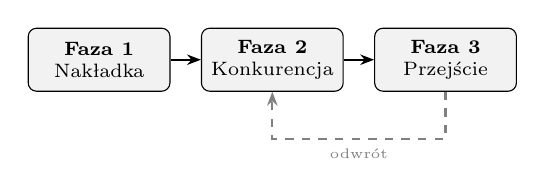
\begin{tikzpicture}[
    phase/.style={draw, rounded corners=3pt, minimum width=1.8cm, minimum height=0.8cm, align=center, font=\scriptsize, fill=black!5},
    arr/.style={-{Stealth[length=5pt]}, thick}
]
\node[phase] (p1) at (0,0) {\textbf{Faza 1}\\Nakładka};
\node[phase] (p2) at (2.2,0) {\textbf{Faza 2}\\Konkurencja};
\node[phase] (p3) at (4.4,0) {\textbf{Faza 3}\\Przejście};

\draw[arr] (p1) -- (p2);
\draw[arr] (p2) -- (p3);
\draw[arr, dashed, gray] (p3.south) -- ++(0,-0.6) -| node[below,font=\tiny,pos=0.25] {odwrót} (p2.south);
\end{tikzpicture}
\caption{Trzyfazowa migracja---odwracalna na każdym etapie.}
\label{fig:migration}
\end{figure}

Głównym mechanizmem nacisku jest fiskalny: gdy warunkowi podatnicy osiągną ,,ekonomicznie znaczącą mniejszość $X$''---grupę na tyle dużą, że represja wobec niej powoduje nietrywialne szkody gospodarcze, a obywatelskie nieposłuszeństwo staje się wiarygodną groźbą---państwo przystępuje do negocjacji. Dla ilustracji przyjmujemy $X \approx 15\%$ PKB, ale rzeczywisty próg zależy od konkretnej gospodarki.

% ============================================================
% 10. SECURITY ANALYSIS
% ============================================================
\section{Analiza bezpieczeństwa}

Rozważamy pięć kategorii przeciwników: indywidualnych złych aktorów, zorganizowane grupy, przeciwników korporacyjnych, przeciwników na poziomie państwa oraz przeciwników na poziomie protokołu.

\textbf{Odporność na atak Sybil}~\cite{douceur2002}. Budowanie reputacji wymaga trwałej, weryfikowalnej interakcji. Koszt udanego ataku Sybil rośnie liniowo wraz z liczbą fałszywych tożsamości i kwadratowo wraz z docelowym poziomem reputacji. Obsługiwanie wielu DID równolegle jest możliwe, lecz z założenia kosztowne---każda tożsamość musi niezależnie gromadzić reputację poprzez rzeczywistą aktywność. W wolnych społeczeństwach koszt ten zniechęca do przypadkowych nadużyć; w dyktaturach równoległe DID stają się narzędziem przetrwania, umożliwiającym podzielony na przedziały opór, podziemną koordynację i bezpieczniejszą nawigację po czarnym rynku.

\textbf{Obrona przed zmową.} Wzorce wzajemnego popierania w zamkniętych grupach są wykrywalne poprzez analizę grafu społecznego. Funkcje agregacji reputacji dyskontują twierdzenia z ciasno zgrupowanych źródeł.

\textbf{Przeciwnik na poziomie państwa.} Trasowanie onion, brak scentralizowanej infrastruktury i rozproszenie roli Weryfikatora wśród bazy uczestników zapewniają, że stłumienie wymaga środków nieproporcjonalnych do jakiejkolwiek korzyści.

\textbf{Prywatność wobec rozliczalności.} Pseudonimowość---środek pośredni między anonimowością a ujawnieniem tożsamości---pozwala DID gromadzić znaczącą reputację bez ujawniania rzeczywistej tożsamości Posiadacza.

% ============================================================
% 11. PRIVACY
% ============================================================
\section{Rozważania dotyczące prywatności}

Model prywatności RSN opiera się na pseudonimowości. Posiadacz kontroluje ujawnianie tożsamości: minimalne (czysty pseudonim), selektywne (powiązanie konkretnych poświadczeń) lub pełne (przypisanie tożsamości prawnej). Opublikowane twierdzenia są trwałe---system wspiera korektę kontekstową, ale nie usunięcie. Posiadacz może porzucić skompromitowany DID i zacząć od nowa, tracąc zgromadzoną reputację.

% ============================================================
% 12. RELATED WORK
% ============================================================
\section{Prace pokrewne}

Specyfikacja W3C DID Core~\cite{did2022} i sieć Ceramic~\cite{ceramic2023} zapewniają fundament tożsamości. EigenTrust~\cite{kamvar2003} zademonstrował rozproszoną agregację reputacji bez centralnego autorytetu. SBT~\cite{weyl2022} wprowadziły nieprzenoszalne tokeny społeczne. RSN różni się naciskiem na koszt ekonomiczny jako filtr jakości oraz mechanizmem wyceny radykalizmu.

DAO~\cite{buterin2014} i głosowanie kwadratowe~\cite{buterin2019} wykazały wykonalność zdecentralizowanego zarządzania. RSN wyprowadza konsensus z dwustronnych negocjacji cenowych, a nie z głosowania.

Propozycja czerpie z teorii anarchokapitalistycznej~\cite{rothbard1973,hoppe2001} w zakresie prywatnego świadczenia usług, lecz odchodzi od niej w dwóch kluczowych aspektach: projektuje z myślą o złośliwości i impulsach odwetowych, zamiast zakładać racjonalność, oraz proponuje stopniową transformację zamiast rewolucji. Koncepcja emergentnych umów społecznych ma poprzedników w Hayekowskiej teorii spontanicznego porządku~\cite{hayek1973}.

\textbf{Anarcho-agoryzm.} RSN dzieli znaczną wspólną płaszczyznę z agorystyczną kontr-ekonomią~\cite{konkin2006}---szczególnie nacisk na budowanie równoległych instytucji i dobrowolną wymianę. Agoryzm skłania się jednak do zakładania racjonalnego interesu własnego jako wystarczającego mechanizmu koordynacji i często brakuje mu konkretnej ścieżki migracji z istniejących struktur państwowych. RSN wyraźnie uwzględnia nieracjonalne skłonności behawioralne i zapewnia fiskalny mechanizm nacisku dla stopniowej transformacji.

\textbf{Merytokracja.} RSN może stanowić pierwszy funkcjonalny opis tego, jak merytokracja~\cite{young1958} może wyłonić się jako właściwość systemowa, a nie slogan. Tradycyjne systemy merytokratyczne zawodzą, ponieważ wymagają centralnego autorytetu do zdefiniowania i egzekwowania ,,zasługi''. W RSN zasługa wyłania się z dwustronnych ocen: ci, którzy dostarczają wartość, gromadzą reputację; żaden komitet nie decyduje, kto ma zasługę.

\textbf{Własność jako przywilej.} RSN fundamentalnie odchodzi od anarchokapitalistycznych i austriackich ujęć praw własności jako naturalnych i absolutnych. W ramach RSN własność jest \emph{przywilejem}---społecznym uznaniem, które w skrajnych przypadkach może zostać wycofane przez wspólnotę, gdy uczestnik fundamentalnie narusza wspólne normy (zdrada, odmowa obrony wspólnoty w kryzysie egzystencjalnym, systematyczne wyzyskiwanie). Nie jest to państwowe wywłaszczenie, lecz wycofanie społecznego uznania przez sieć relacji dwustronnych.

% ============================================================
% 13. LIMITATIONS
% ============================================================
\section{Dyskusja i ograniczenia}

\textbf{Zimny start.} Wartość RSN zależy od efektów sieciowych; wcześni użytkownicy napotykają ograniczoną wartość, dopóki uczestnictwo nie osiągnie progu. Jednak nawet na wczesnych etapach sieć DID służy jako użyteczne uzupełniające źródło informacji. Oczekuje się, że wczesna ocena reputacji i ocena autorytetów będą rozwijać się stopniowo, wraz z rosnącym wyrafinowaniem.

\textbf{Zapobieganie pasożytnictwu i kontrola dostępu.} Docelowe DID mogą nakładać stopniowalne opłaty i ograniczenia dostępu na zapytania od DID o niskiej reputacji. Nie jest to binarne, lecz ciągła skala: im mniej reputacji ma odpytujący DID, tym mniej informacji otrzymuje, tym dłużej czeka i tym więcej płaci. Mechanizm ten motywuje do rzeczywistego uczestnictwa zamiast biernej konsumpcji.

\textbf{Nierówność dostępu.} Koszt publikowania twierdzeń może odfiltrowywać uzasadnione skargi od uczestników znajdujących się w gorszej sytuacji ekonomicznej. Łagodzenie: każdy uczestnik jednocześnie pełni rolę potencjalnego weryfikatora (lub deleguje tę rolę) i zarabia opłaty weryfikacyjne. W wystarczająco długim horyzoncie czasowym nieradykalny uczestnik powinien zbliżyć się do neutralności finansowej---dochód z weryfikacji w przybliżeniu rekompensujący koszty publikacji. Jest to oczekiwanie statystyczne, a nie gwarancja.

\textbf{Nierówność reputacji.} Wcześni użytkownicy gromadzą przewagi, które mogą tworzyć bariery dla późniejszych. Jednak ocena reputacji jest wykonywana przez zewnętrznych dostawców, którzy mogą zdecydować się łagodzić przewagę pierwszeństwa poprzez swoje algorytmy agregacji. Bycie pierwszym z dobrą reputacją jest uprawnioną komparatywną przewagą ekonomiczną---i to z założenia.

\textbf{Pytania otwarte.} Optymalne funkcje kosztów, standardy agregacji, zarządzanie protokołem oraz interakcja z syntetycznymi danymi reputacyjnymi generowanymi przez AI pozostają obszarami przyszłych prac.

Niniejsza praca nie twierdzi, że RSN będzie wytwarzać optymalne rezultaty we wszystkich okolicznościach. Twierdzi, że RSN stanowi \emph{wykonalną} alternatywę---technicznie implementowalną, ekonomicznie samopodtrzymującą się i społecznie zgodną ze skłonnościami behawioralnymi człowieka takimi, jakie są w rzeczywistości.

% ============================================================
% 14. CONCLUSION
% ============================================================
\section{Wnioski}

Niniejsza praca przedstawiła Reputacyjną Sieć Społeczną, zdecentralizowany protokół umożliwiający pseudonimową, weryfikowalną wymianę reputacji. Zasada Kosztownego Radykalizmu zapewnia, że oszukańcze twierdzenia są wyceniane poza zasięg bez cenzury. Zaproponowana ścieżka migracji umożliwia stopniowe, odwracalne przejście z istniejących instytucji. Projekt uwzględnia ludzką naturę taką, jaka jest---w tym małostkowość, złośliwość i pragnienie satysfakcji z odwetu---zamiast wymagać transformacji ideologicznej. Rezultatem nie jest utopia, lecz system, w którym sprawiedliwość jest dostępna, reputacja jest zasłużona, a koszt występku ponosi strona, która go spowodowała.

% ============================================================
% REFERENCES
% ============================================================
\bibliography{references}

\end{document}
